%% !TEX root =  paper.tex
\section{Approach}\label{sec:approach}

The goal of our approach is to automatically find potential fixes that can repair a broken web test that was used to work correctly on a  version $k$ of the AUT, and that now fails when applied on a subsequent version $k+n$ (with $n>1$).

The focus of our technique is to repair \textit{locators}, that represent the main source of breakage.
Our technique can detect and correct locator problems that pertain to the breakage scenarios described in \autoref{sec:breakage-scenarios}. A main assumption of our work is that the two web applications object of our analysis are correct, i.e., do not contain bugs that make the tests fail. Thus, we ensure that when tests fail to execute is due to actual regressions of the tests. For this reason, in this work, we do not target silent breakages because we assume the software to be correct.

\begin{figure}[t]
\centering
%\fbox{
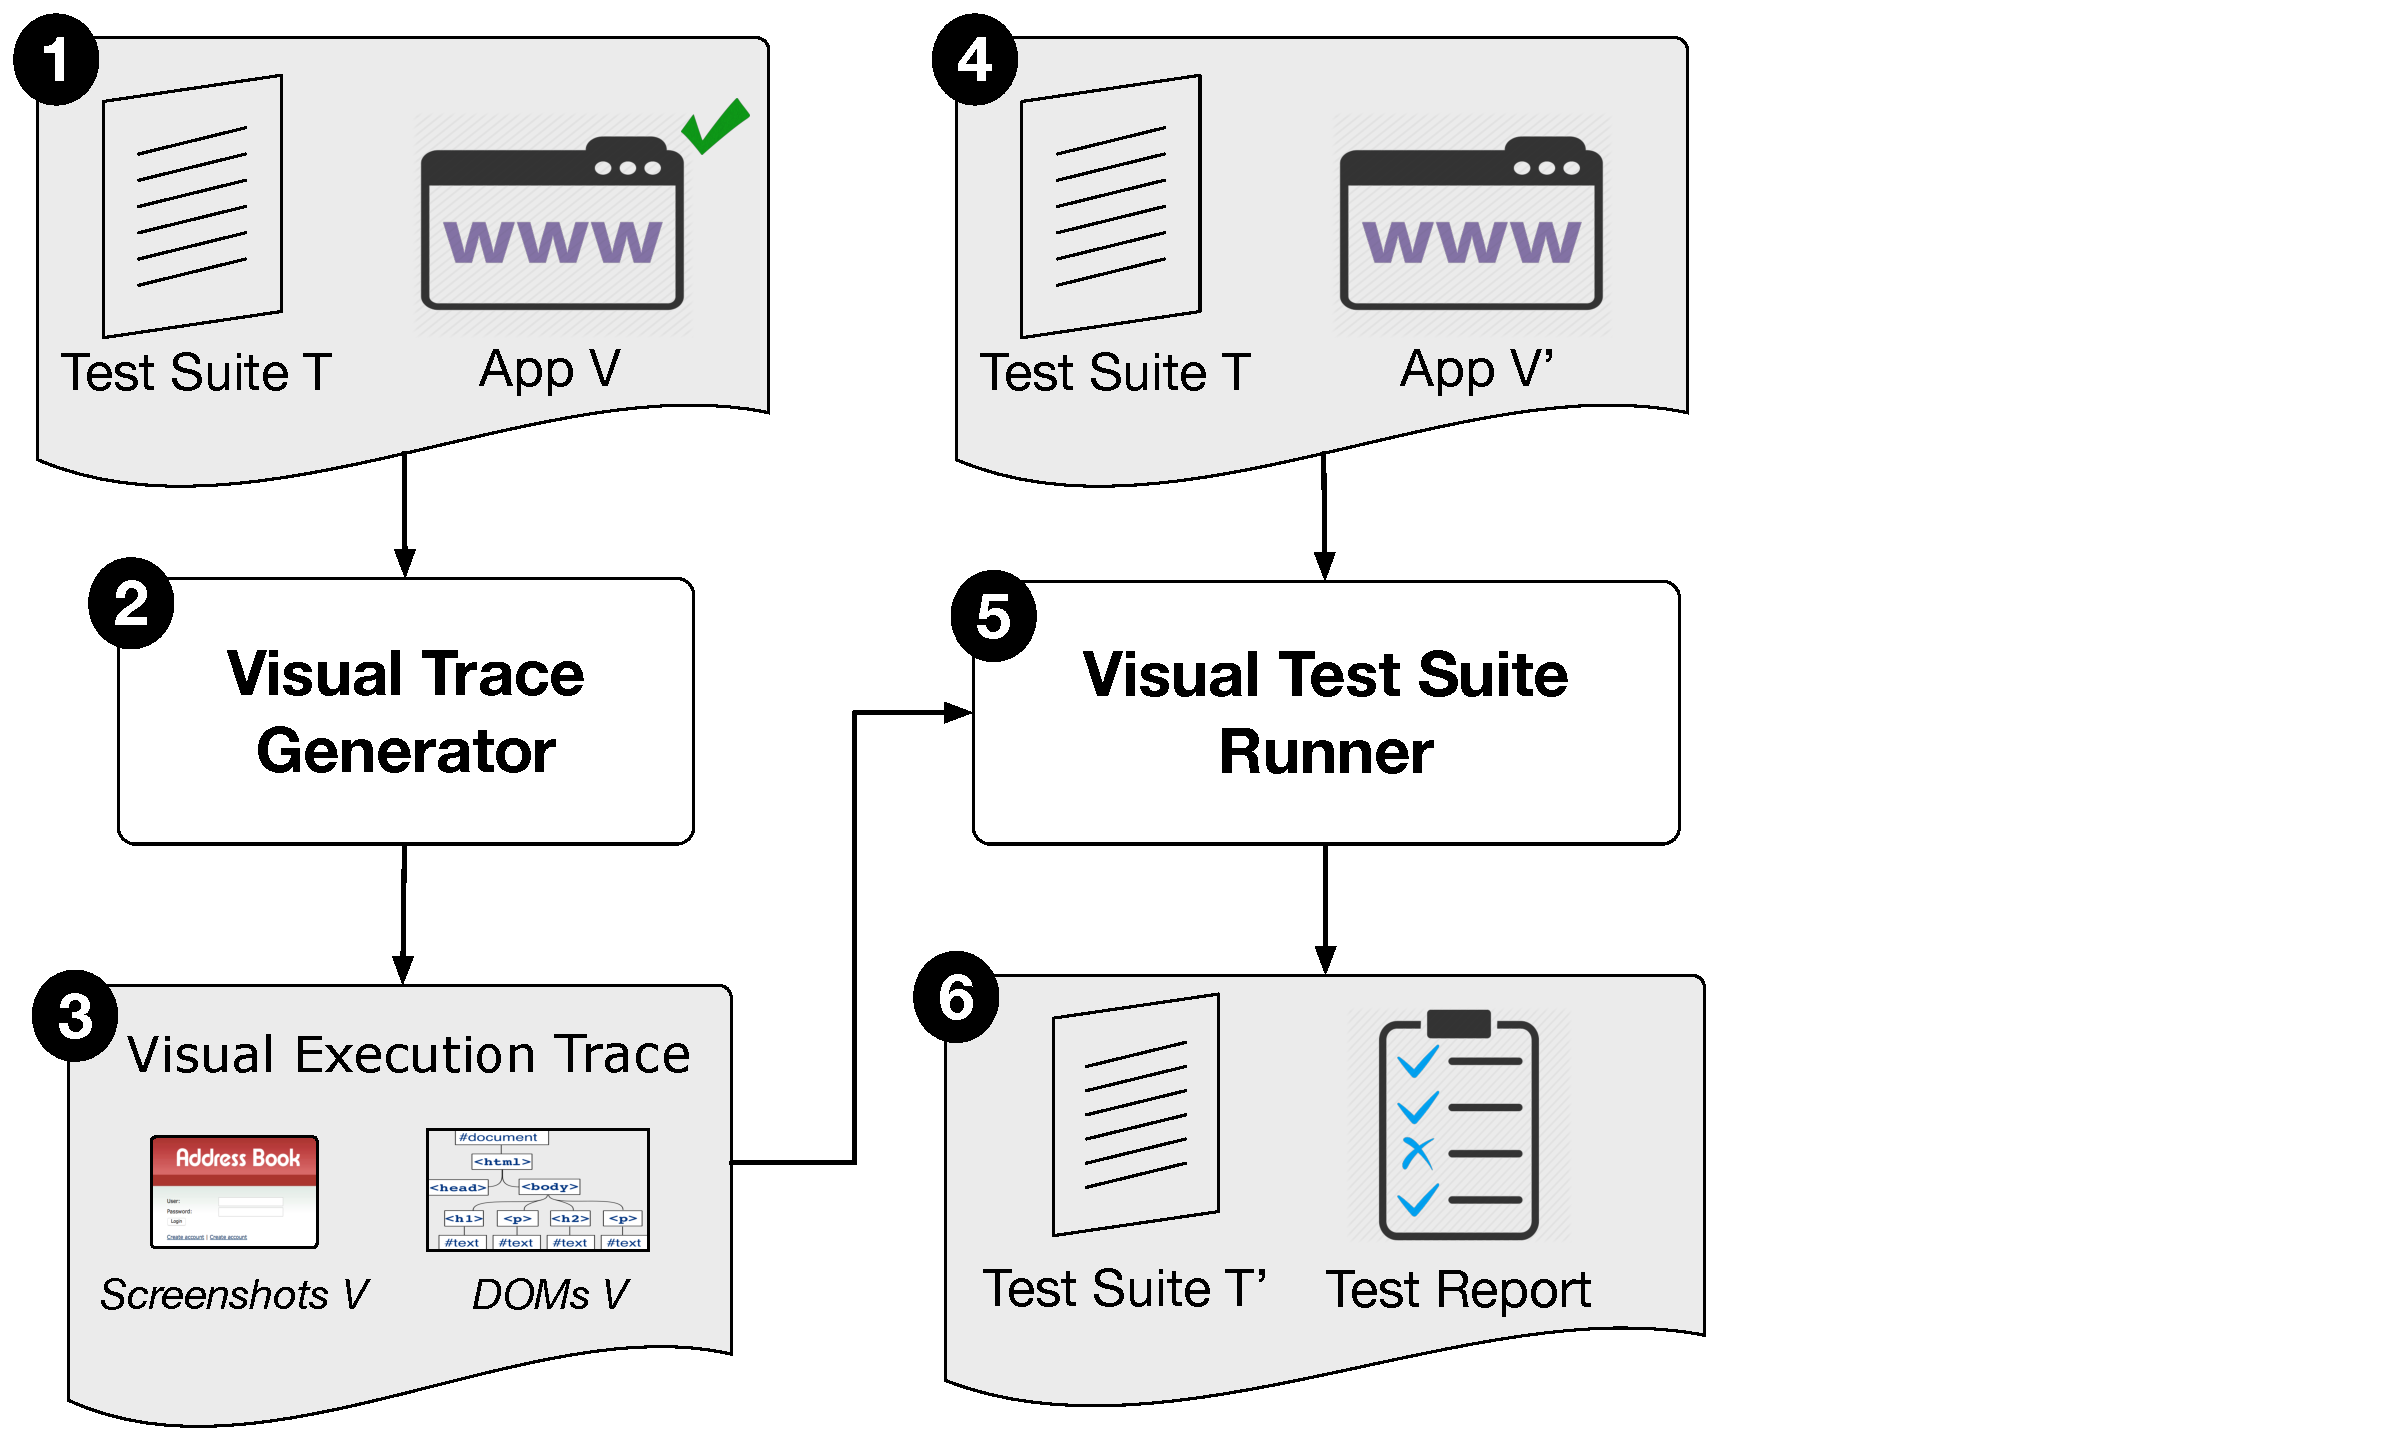
\includegraphics[trim={0.2cm 0cm 11cm 0.2cm},clip,scale=0.25]{images/approach-bigger}
%}
\caption{Overview of our approach. Inputs and outputs are shown as parallelograms, whereas the proposed approach is represented as rounded rectangles. Dotted rectangle depicts manual processes.}
\label{approach}
\end{figure}

\begin{itemize}
\item use SIFT to determine whether the image is present/absent
\item SIFT returns also an estimate of where the majority of keypoints has been found
\item Template matching usually returns multiple or inaccurate results
\item the idea is to filter the TM results with SIFT's
\item one try might be to use multiple images (i.e. both the perfectly cropped and the larger visual locator).
\item try to implement Chamfer Matching
\end{itemize}

\autoref{approach} illustrates the usage scenario for our approach in a real-world testing environment. 
First, given a stable version of the web application $V$ along with its working test suite $T$ (i.e., in which all test pass)~\ding{182}, a tester would run $T$ by means of the first module of \tool, the Visual Trace Generator~\ding{183}. Such a module stores for each test a number of information (e.g., screenshots, DOMs), which constitute the visual execution trace of the tests~\ding{184}. 
Then, when the application $V$ gets modified/evolved, a new version $V'$ is produced~\ding{185}. At this point, a tester may wish to use $T$ to check if regressions have occurred. To this aim, she uses the second module of \tool, the Visual Test Suite Runner~\ding{186}. Such a module runs each test case of the the test suite $T$ against the new version $V'$, and makes use of the visual execution trace previously saved to verify the correctness of each test statement, and eventually attempt to repair locator breakages at runtime in an \textit{online mode}. At the end of the process, \tool outputs the new verified (and eventually corrected) test suite $T'$ that works on $V'$, together with report information. 
The developer can hence manually analyse the report to decide on the correctness of the test cases. The manual effort required is potentially significantly reduced in comparison to a user carefully verifying each executing test and manually searching for fixes as breakages occur. If any such issues exist, then the process outputs a repaired test, that the developer can inspect and accept or fix  manually before moving on. If the developer decides that there are no unintended side effects, then $T$ can
be updated to $T'$, as any subsequent app changes need to be tested against the most recent version of the test suite.

We now detail each the steps of our approach.

\head{Visual Trace Collection}

The first module of \tool consists 

\head{Visual Test Suite Runner}


%\IncMargin{0.5em}
%\begin{algorithm}[h]
%\scriptsize
%\SetAlgoLined
%\KwResult{Write here the result}
% initialization\;
% \While{While condition}{
%  instructions\;
%  \eIf{condition}{
%   instructions1\;
%   instructions2\;
%   }{
%   instructions3\;
%  }
% }
% \caption{How to write algorithms}
%\end{algorithm}\DecMargin{1em}

\subsection{Implementation}\label{sec:implementation}

We implemented our approach in a tool called \tool, which is publicly available (URL omitted). 
The tool is written in Java, and supports Selenium test suites written in Java. However, our overall approach is more general and applicable to test suites developed using other programming languages or testing frameworks. 
\tool gets as input the path to the test suites, collects the visual execution traces by means of an AspectJ module, and runs the visual repair algorithms. 
\tool makes use of the traces to generate potential repairs and generates a list of repaired test cases.

\head{Requirements and Limitations}

A running requirement is that the browser needs to be displayed and the web elements rendered on the screen (i.e., headless browsers such as PhantomJS are currently not supported).

A limitation is that the tests numbers need to be synchronized between the two versions. \andrea{Rahul: how do we deal with that when we added/removed statements?}







